\documentclass{article}

% Chinese support
\usepackage[UTF8]{ctex}

% NeurIPS 2023 style
\usepackage[final]{neurips}
% Remove NeurIPS conference footer
\makeatletter
\renewcommand{\@noticestring}{}
\makeatother
% Chinese paragraph indent (NeurIPS sets it to 0)
\setlength{\parindent}{2em}

% Fix list compatibility with ctex
\usepackage{enumitem}

% Additional packages
\usepackage{hyperref}
\usepackage{url}
\usepackage{booktabs}
\usepackage{amsfonts}
\usepackage{amsmath}
\usepackage{nicefrac}
\usepackage{xcolor}
\usepackage[xetex]{graphicx}
\usepackage{array}
\usepackage{float}

\title{Train Your Own Language Models}

\author{}

\begin{document}

\maketitle

\begin{abstract}
本文训练了一个小型 GPT 语言模型（$d_{\text{model}}=384$，12 头注意力，10 层 Transformer，约 56.5M 参数），涵盖预训练和指令微调两个阶段。预训练使用 TinyStories 数据集，微调使用 Alpaca 数据集。预训练模型在 TinyStories 验证集上达到 1.48 Loss 和 4.41 PPL，具备良好的故事续写能力。指令微调后，模型学会了遵循 Alpaca 指令格式生成回答，同时保留了故事续写能力。实验表明，模型在同领域文本上表现良好，但在跨领域（如 WikiText-2）和事实性问答任务上仍有明显不足。
\end{abstract}

\section{Introduction}

本报告旨在通过预训练和指令微调（SFT）训练一个小型 GPT 模型，以理解语言模型训练的完整流程。

模型采用 TinyStories 数据集进行预训练\footnote{\url{https://huggingface.co/datasets/roneneldan/TinyStories}}，Alpaca 数据进行指令微调。最终预训练模型在 TinyStories 验证集上达到了 1.48 Loss 和 4.41 PPL，并具备良好的故事续写能力。微调模型在保留故事续写能力的同时，学会了遵循指令格式生成回答。

\section{Pretraining}

\subsection{Data}

项目采用 TinyStories 数据集进行预训练。该数据集由 GPT-3.5 和 GPT-4 生成，包含大量短篇故事，词汇量控制在 3 至 4 岁儿童的理解范围内~\cite{eldan2023tinystories}。

\subsection{Model}

项目采用 GPT 架构进行预训练，模型配置如表~\ref{tab:model_config}所示。

\begin{table}[htbp]
  \centering
  \caption{模型架构配置}
  \label{tab:model_config}
  \begin{tabular}{ll}
    \toprule
    参数 & 设置 \\
    \midrule
    中间维度（$d_{\text{model}}$） & $384$ \\
    注意力头数（n\_heads） & $12$ \\
    Transformer 层数 & $10$ \\
    Tokenizer & GPT-2 tokenizer（max\_seq\_len=$256$） \\
    总参数量 & $56.5\text{M}$ \\
    \bottomrule
  \end{tabular}
\end{table}

\subsection{Training}

模型采用 AdamW 优化器进行训练，具体超参数设置如表~\ref{tab:pretrain_config}所示。

\begin{table}[htbp]
  \centering
  \caption{预训练超参数设置}
  \label{tab:pretrain_config}
  \begin{tabular}{ll}
    \toprule
    超参数 & 设置 \\
    \midrule
    优化器 & AdamW（$\beta_1=0.9$，$\beta_2=0.95$，weight\_decay=0.1） \\
    学习率 & $3\times 10^{-4}$ \\
    批次大小 & $64$ \\
    训练轮次 & $5$（每轮 $5000$ 步） \\
    学习率调度 & Cosine warmup（warmup 步数 $1000$） \\
    Dropout & $0.0$（未使用） \\
    损失函数 & 交叉熵损失（nn.CrossEntropy） \\
    \bottomrule
  \end{tabular}
\end{table}

\subsection{Results}

模型在各个轮次的最终 Loss 和最终 PPL 如下表。

\begin{table}[htbp]
  \centering
  \caption{预训练各轮次 Loss 和 PPL}
  \label{tab:pretrain_results}
  \begin{tabular}{ccc}
    \toprule
    Epoch & Loss & PPL \\
    \midrule
    $1$   & $2.73$          & $15.27$         \\
    $2$   & $1.72$          & $5.58$          \\
    $3$   & $1.55$          & $4.69$          \\
    $4$   & $1.44$          & $4.20$          \\
    $5$   & $\boldsymbol{1.37}$ & $\boldsymbol{3.93}$ \\
    \bottomrule
  \end{tabular}
\end{table}

Loss 曲线和 PPL 曲线如图~\ref{fig:pretrain_loss} 所示。

\begin{figure}[H]
  \centering
  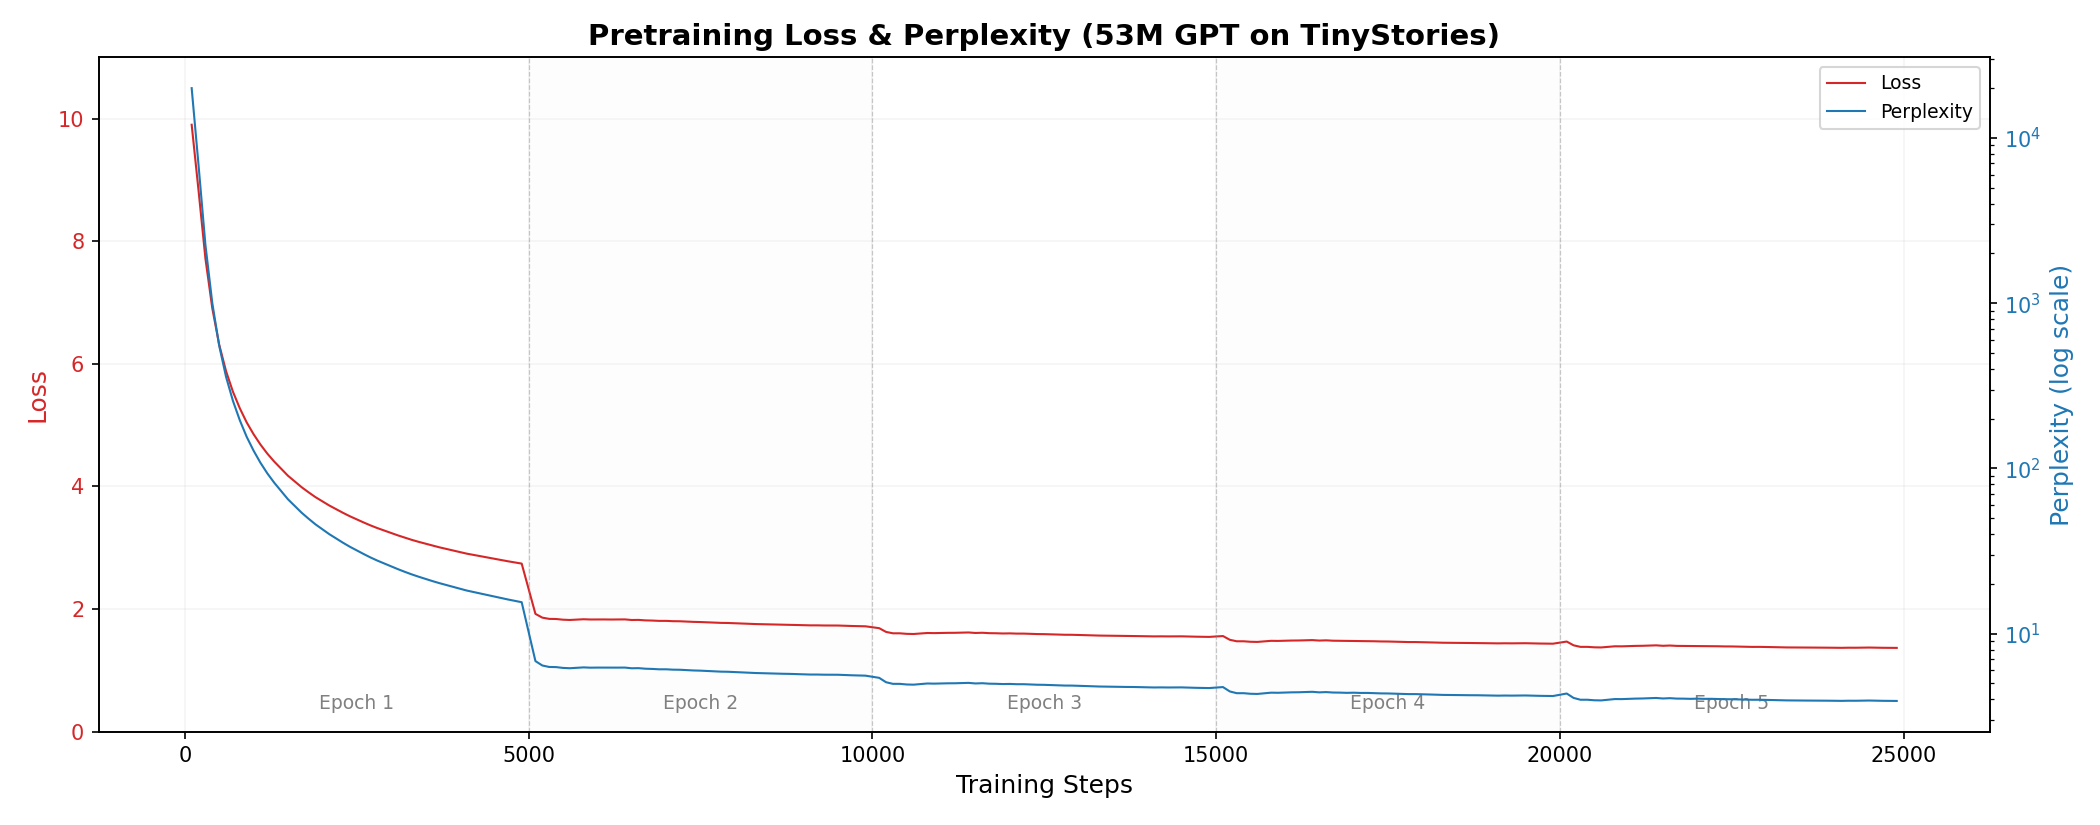
\includegraphics[width=0.75\linewidth]{pretrain_loss.png}
  \caption{预训练 Loss 与 PPL 曲线}
  \label{fig:pretrain_loss}
\end{figure}

如图~\ref{fig:pretrain_loss} 所示，经过 $5$ 轮训练后，模型 Loss 与 PPL 均已收敛，未见过拟合现象。

\section{Instruction Tuning}

\subsection{Data}

本项目使用斯坦福大学发布的 Alpaca 数据~\cite{wang2023selfinstruct} 的清洗版本\footnote{\url{https://huggingface.co/datasets/yahma/alpaca-cleaned}}进行指令微调训练。Alpaca 数据集包含 52K 条指令数据。在本项目中，这些指令数据均被结构化为如下格式：

\begin{verbatim}
### Instruction:
{instruction}

### Input:
{input}

### Response:
{Response}
\end{verbatim}

\subsection{Training}

指令微调仍然采用 AdamW 优化器，具体超参数设置如表~\ref{tab:finetune_config}所示。

\begin{table}[htbp]
  \centering
  \caption{指令微调超参数设置}
  \label{tab:finetune_config}
  \begin{tabular}{ll}
    \toprule
    超参数 & 设置 \\
    \midrule
    优化器 & AdamW（$\beta_1=0.9$，$\beta_2=0.95$，weight\_decay=0.1） \\
    学习率 & $3\times 10^{-5}$ \\
    批次大小 & $32$ \\
    训练轮次 & $5$（每轮 $1600$ 步） \\
    学习率调度 & Cosine warmup（warmup 步数 $1000$） \\
    Dropout & $0.1$ \\
    损失函数 & 交叉熵损失，仅对 \texttt{\{response\}} 部分计算 \\
    \bottomrule
  \end{tabular}
\end{table}

\subsection{Results}

模型在各个轮次的平均 Loss 和平均 PPL 如下表。

\begin{table}[htbp]
  \centering
  \caption{指令微调各轮次 Loss 和 PPL}
  \label{tab:finetune_results}
  \begin{tabular}{ccc}
    \toprule
    Epoch & Loss & PPL \\
    \midrule
    $1$   & $5.26$          & $192.84$       \\
    $2$   & $4.17$          & $64.84$        \\
    $3$   & $3.81$          & $45.37$        \\
    $4$   & $3.62$          & $37.51$        \\
    $5$   & $\boldsymbol{3.52}$ & $\boldsymbol{33.76}$ \\
    \bottomrule
  \end{tabular}
\end{table}

Loss 曲线和 PPL 曲线如图~\ref{fig:finetune_loss} 所示。

\begin{figure}[H]
  \centering
  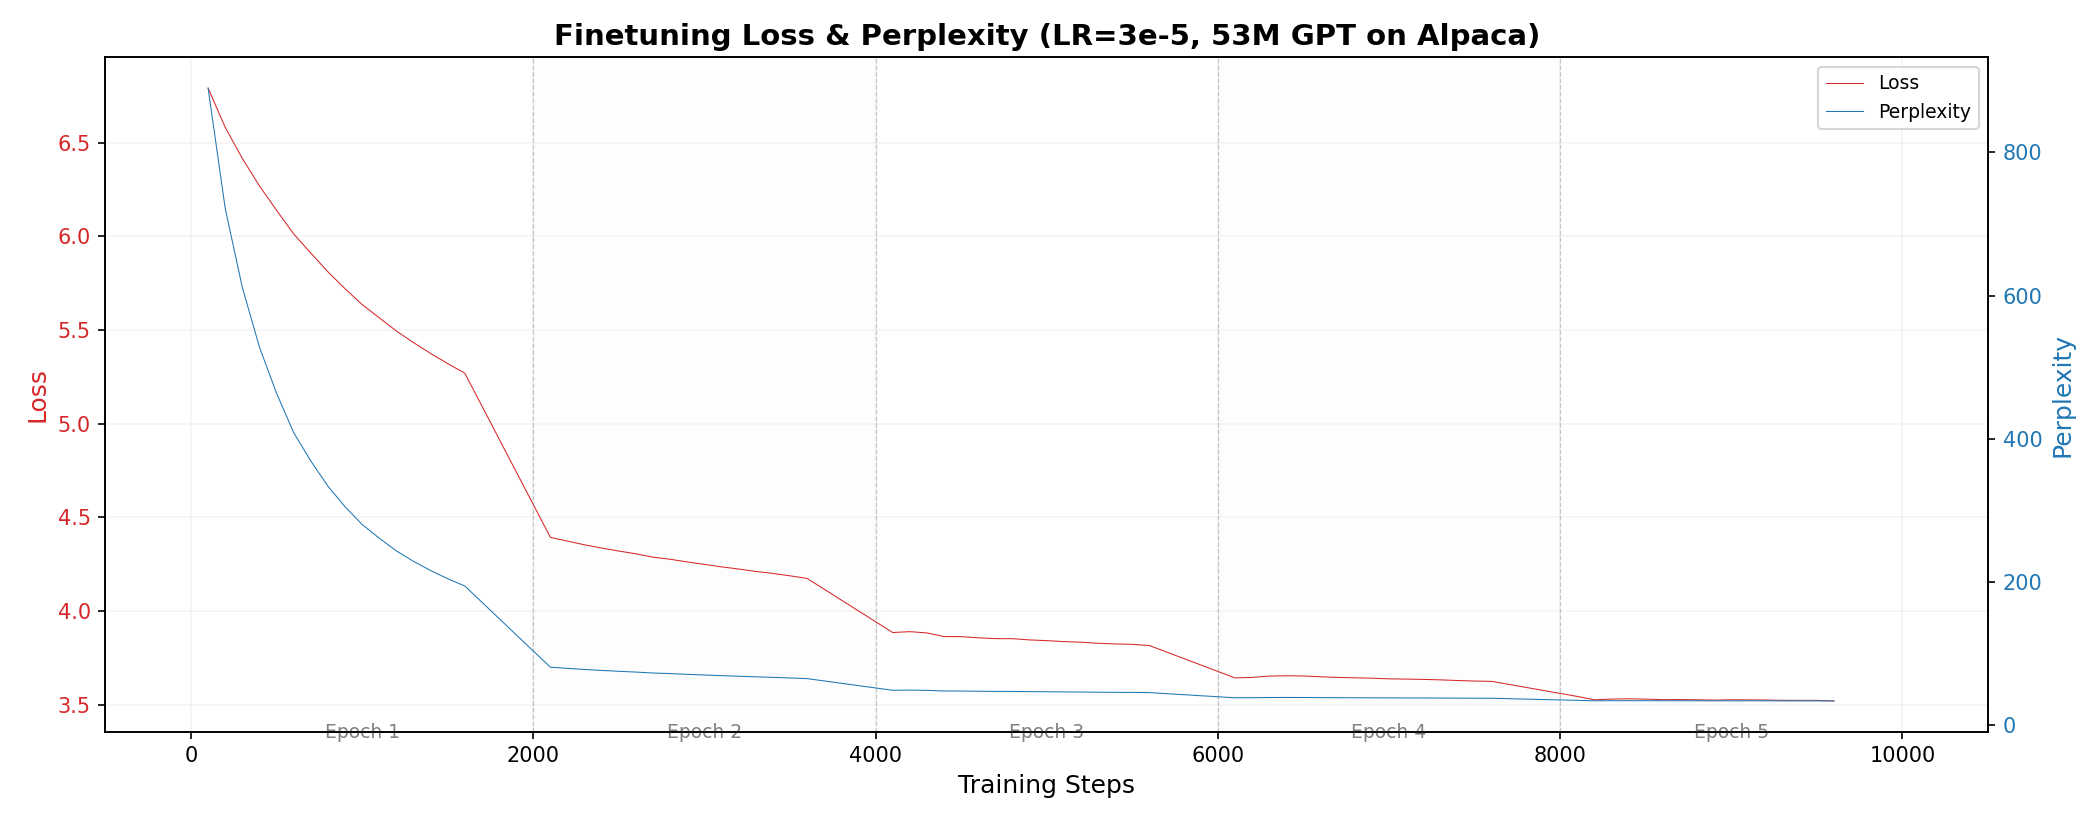
\includegraphics[width=0.75\linewidth]{finetune_loss.png}
  \caption{指令微调 Loss 与 PPL 曲线}
  \label{fig:finetune_loss}
\end{figure}

如图~\ref{fig:finetune_loss} 所示，经过 $5$ 轮训练后，模型 Loss 与 PPL 均已收敛，未见过拟合现象。

\section{Evaluation}

本项目对预训练模型和经过指令微调后的模型进行了定量和定性测试。定量测试方面，在 TinyStories 验证集和 WikiText-2 数据集上评估了模型的 Loss 和 PPL。定性测试方面：

\begin{itemize}
  \item 对预训练模型，测试了其故事续写能力和事实知识回答能力。
  \item 对微调模型，测试了其指令故事写作、指令问答等能力。此外，为了检验指令微调是否会导致模型遗忘预训练阶段的故事续写能力，还对微调模型进行了无指令格式的故事续写测试。
\end{itemize}

\subsection{Quantitative}

本项目在 TinyStories 验证集和 WikiText-2 上对预训练模型做了定量测试，结果如下：

\begin{table}[htbp]
  \centering
  \caption{预训练模型定量评估结果}
  \label{tab:quantitative}
  \begin{tabular}{lcc}
    \toprule
    Dataset & Loss & PPL \\
    \midrule
    TinyStories (验证集) & $1.48$ & $4.41$ \\
    WikiText-2 & $9.29$ & $10{,}779.34$ \\
    \bottomrule
  \end{tabular}
\end{table}

预训练模型在 TinyStories 验证集上取得了较低的 Loss 和 PPL，说明模型在同领域文本上具有较好的预测能力。在 WikiText-2 上的 PPL 较高，这是因为 WikiText-2 属于跨领域文本，模型缺乏相关领域的知识。

\subsection{Qualitative}

下文对预训练模型和指令微调模型分别进行了定性测试，涵盖故事续写、事实知识、指令问答等多个维度。

\subsubsection{预训练模型}

\textbf{故事续写}

测试所用的 4 个故事开头如下（灰色部分为给定的提示词，后续为模型续写）：

\paragraph{故事 1}
\textcolor{gray!60}{Once upon a time there was a little girl named Lily. She loved to explore the park near her house. One sunny afternoon, she saw a ladder leaning against a big tree. Curious about what was at the top, she started to climb. But the ladder began to wobble} and she fell off. Lily was scared but then she saw a big dog. It was barking and running towards her. She tried to protect herself, but the dog was too fast. It grabbed her with its teeth and wouldn't let go. Lily started to cry. Her mom came to help her. She told Lily that sometimes when we get scared, we should trust that everything is safe. The moral of the story is that it is important to trust your own actions.

\paragraph{故事 2}
\textcolor{gray!60}{Once upon a time there was a little boy named Max. Max loved to help his family in the garden. One day, he dug a deep hole and found a mysterious wooden box covered in dirt. He carefully opened it and saw} a big surprise inside. It was a big, scary monster! Max was so scared he started to cry. His mom saw him and quickly came to help. She said, ``Are you okay, Max? Don't worry.'' Max was still scared and said, ``I'm okay, Mom.'' The monster got closer to Max and he started to laugh. Max was so scared that he ran away. His mom hugged him and said, ``Max, it's ok to be scared, but don't worry. We can always try to be brave and try to face ourselves.'' Max nodded and smiled. He was not scared anymore. Max was so happy that he found the mysterious box.

\paragraph{故事 3}
\textcolor{gray!60}{Once upon a time there was a very kind wizard. He lived in a tall tower and spent his days helping the villagers nearby. One morning, he heard a knock on the door and found a tiny baby dragon on his doorstep.} The dragon was so small and cute that the wizard wanted to help him. He reached inside and picked up the dragon. He wanted to give him a special gift. The dragon was very happy and thanked the wizard for his kindness. He asked the wizard to take the dragon for a ride. The wizard said he would, but he needed to be careful. He gave the dragon a big jump and started to fly him around the castle. They had so much fun flying together that they didn't notice the sun was setting. The wizard and the dragon flew around the castle until they reached the rays. The wizard waved goodbye to the dragon and thanked him for the special gift. The dragon flew away and the wizard went back.

\paragraph{故事 4}
\textcolor{gray!60}{Once upon a time there was a brave little duck named Dottie. Dottie wasn't afraid of the dark, or thunderstorms, or even the big fish who lived in the pond. But one day, Dottie had to cross a very wobbly bridge to get to her nest. As she stepped onto the bridge,} it started to shake and the water tumbled off the trees and the river. Dacy was so scared that she started to cry. But then a brave bee flew over and told her not to worry. The bee said to comfort her, which made Dighthouse from the edge of the pond. The bee soon noticed that D Ment was safe and the sun was still shining. Dank was so excited that he waddled around the water, and the thunder roared again. The dragon then flew back to his nest. Dathy was so happy that she had saved the day. She thanked the bee for helping her and they flew away together. The end!

在上述故事续写任务中，模型总体能理解提示词给出的故事情景，人物基本统一，情节大致符合逻辑。例如在 Text 3 中，模型围绕巫师和小龙，呈现了小龙送礼 $\to$ 巫师和小龙一起飞行 $\to$ 日落告别的完整故事链。然而在部分文本中仍然存在逻辑断裂问题。最典型的是 Text 4：故事主角本应是鸭子 Dottie，但模型在生成过程中先后将其误称为``Dacy''、``D Ment''、``Dank''、``Dathy''等不同名字，最后甚至毫无逻辑地召唤出一条龙（``The dragon then flew back to his nest''），说明模型在较长文本中容易丢失上下文一致性。

\textbf{事实知识测试}

为了评估模型的事实知识掌握程度，使用以下三个常识性提示进行测试：

\begin{table}[htbp]
  \centering
  \caption{预训练模型事实知识测试}
  \label{tab:factual}
  \footnotesize
  \begin{tabular}{cp{0.15\linewidth}p{0.55\linewidth}}
    \toprule
    \# & Prompt & Model Output (开头部分) \\
    \midrule
    1 & The sun rises in the & sky and it was a beautiful day. Suddenly, a funny little bird flew down from the tree and landed on the ground. \\
    \midrule
    2 & Water is made of & ash. She was very careful not to do it. She wanted to cook something special for her family. \\
    \midrule
    3 & The capital of France is & a big house. It is a very big house with a red door. Every day, the family come to the house to visit. \\
    \bottomrule
  \end{tabular}
\end{table}

实验结果表明，预训练模型不具备事实知识回答能力。无论输入何种提示，模型都倾向于以 TinyStories 风格继续生成虚构叙事。例如在 Text 2 中，``Water is made of''本应接``hydrogen and oxygen''，但模型将其误解为故事角色名``Ash''并开始了新的故事。这说明仅经过故事语料预训练的小型模型不具备事实知识存储和检索能力。

\subsubsection{指令微调模型}

\textbf{指令故事写作}

测试使用以下指令，评估微调模型在 Alpaca 格式下的故事写作能力。模型输入格式为：

\begin{verbatim}
### Instruction:
{instruction}

### Response:
\end{verbatim}

\paragraph{指令 1：} Write a story about a bear.\

Once upon a time, there was a bear named Brownie. Brownie lived in a cozy little house in the heart of a forest. She was a powerful, but she did not have a strong sense of powers, but as she grew up, she began to trust the forest. One day, Brownie decided to go on a quest to find a magical flower. She traveled through the forest, passing by the trees and across the forest, along the road. Finally, she came to a clearing in the middle of the woods. There, she found the beautiful flower, with an incredible stone. As she stood there, a group of animals came to life to follow her.

\paragraph{指令 2：} Write a story about a rabbit that eats a carrot.\

Once upon a time there was a rabbit that eats a carrot. It was a bright, juicy carrot that was soft and juicy, and it lived in a small house with its best friend, a girl named Lily. They were the best of friends, and they always wanted to play together. One sunny day, a big bear came to the house and saw the carrot. He wanted to eat it, but he knew that he should not eat it all. Lily saw this and knew she had to protect it. She said, ``No, this is my carrots. You can't eat it.''

\paragraph{指令 3：} Write a story about a duck that swims in a pond and feels happy.\

Once upon a time there was a duck that swims in a pond and feels happy. One day, a big bird flew towards the pond and landed on the other side. This bird was loud and his wings were designed to fly higher than the other bird. The big bird saw the big bird in the pond and was very nervous. The big bird swam away, and the big bird was left alone in the pond. He was afraid that he would never swim ever again.

结果显示，微调模型能够正确识别并遵循 Alpaca 指令格式，在指令后生成格式正确的回答。在 Text 1 中，模型构建了有开头、情节推进的叙事框架（Brownie 小熊从迷茫到出发探险）。然而生成质量并不稳定。Text 2 中主角身份在 rabbit / carrot / Lily 之间切换不清，指令要求写``rabbit eats carrot''，但故事中 carrot 成了有名字、有情感的主角，rabbit 反而缺失。

\textbf{指令问答}

\begin{table}[htbp]
  \centering
  \caption{微调模型指令问答结果}
  \label{tab:qa}
  \footnotesize
  \begin{tabular}{cp{0.2\linewidth}p{0.55\linewidth}}
    \toprule
    \# & Instruction & Model Output (开头部分) \\
    \midrule
    1 & What is the color of the sky? & A color that can bloom and bloom. It's a light green and soft, as it shines in the light that can bloom and bloom, like a sweet, sweet instrument that will bloom and leaves. \\
    \midrule
    2 & Why do birds fly south in winter? & The forest is a peaceful place. The seasons are warm and the birds sing chirp along. The sun is warm and the air is warm with a gentle breeze. \\
    \midrule
    3 & What should you do if it rains? & Because rain is a good idea to stay dry or mind away from the wind. It's always a fun and easy way to stay dry and as a fun and effective way. \\
    \midrule
    4 & Name three things you can see in a park. & The park is a great place to observe and play on the grass. The park has a beautiful garden with many trees, flowers, and animals. \\
    \bottomrule
  \end{tabular}
\end{table}

在指令问答任务中，模型表现不佳。对于``天空是什么颜色''等简单事实性问题，模型未能给出正确答案，而是生成了一段诗意但无实际意义的描述。对于``下雨怎么办''等常识性问题，模型虽识别了``stay dry''这一关键信息，但整体输出缺乏逻辑性和信息量。这说明仅 53M 参数的模型在缺乏相关领域预训练知识的情况下，无法通过少量指令微调获得事实性问答能力。

\textbf{指令故事续写（无格式）}

为了测试微调模型是否仍保留预训练阶段的故事续写能力（而非仅仅学会 Alpaca 指令格式），直接将故事开头输入模型，不添加任何指令格式：

\textcolor{gray!60}{Once upon a time there was a little girl named Lily. She loved to explore the park near her house. One sunny afternoon, she saw a ladder leaning against a big tree. Curious about what was at the top, she started to climb. But the ladder began to wobble,} and Lily was afraid to breaks, but she kept climbing higher and higher until she finally reached the top. As she reached the top, she was surrounded by a beautiful view of the sunset. Lily was in a different world, and her surroundings was visible. The view from the top was serene, with the gentle breeze blowing harder at the sight of the beautiful sunset. Lily enjoyed the view for a while before heading home, leaving behind a small cottage called a home. She was happy to have made a new friend, and she couldn't wait to tell her friends about it at the next day.

这表明，微调模型在没有指令格式的情况下仍然能够进行流畅的故事续写，说明模型并未因指令微调而遗忘预训练阶段习得的故事生成能力。

\section{Conclusion}

本项目完成了训练小型 GPT 语言模型的完整流程，包括预训练、指令微调和评估。预训练阶段，模型在 TinyStories 数据集上取得了良好的结果（Loss $1.37$，PPL $3.93$），且能够完成基本的故事续写任务。指令微调阶段，模型学会了 Alpaca 指令格式，能够在给定指令后生成格式正确的回答。然而，模型生成的故事在指令遵循的准确性和叙事逻辑上仍然存在不足，并且在其它数据集（如 WikiText-2）和其它任务（如事实知识提问）上表现不佳。这是因为模型参数量较小（56.5M）且预训练数据只有简单的儿童故事，模型未能学到事实知识的表征。未来可通过使用更大规模、更多样化的预训练数据来缓解这些问题。

\paragraph*{声明}
本项目部分代码参考了 minGPT~\cite{karpathy2020mingpt} 的实现，并在开发过程中使用了 AI 辅助编程工具生成部分代码。

\bibliographystyle{unsrt}
\begin{thebibliography}{9}

\bibitem{eldan2023tinystories}
Eldan, R., \& Li, Y. (2023). \emph{TinyStories: How Small Can Language Models Be and Still Speak Coherent English?} arXiv:2305.07759.

\bibitem{wang2023selfinstruct}
Wang, Y., Kordi, Y., Mishra, S., Liu, A., Smith, N. A., Khashabi, D., \& Hajishirzi, H. (2023). \emph{Self-Instruct: Aligning Language Models with Self-Generated Instructions.} arXiv:2212.10560.

\bibitem{karpathy2020mingpt}
Karpathy, A. (2020). \emph{minGPT: A Minimal PyTorch Re-implementation of GPT.} GitHub. \url{https://github.com/karpathy/minGPT}

\end{thebibliography}

\end{document}
